\documentclass[conference]{IEEEtran}
\usepackage[utf8]{inputenc}
\usepackage[T1]{fontenc}
\usepackage{amsmath,amssymb,amsfonts,mathtools}
\usepackage{graphicx,booktabs,colortbl,xcolor,url,array}
\usepackage{hyperref}
\definecolor{navy}{HTML}{1E3A8A}
\definecolor{medblue}{HTML}{3B82F6}
\definecolor{lightblue}{HTML}{EFF6FF}
\definecolor{lavender}{HTML}{F5F3FF}
\definecolor{deeppurple}{HTML}{5B21B6}
\hypersetup{colorlinks=true,linkcolor=navy,citecolor=deeppurple,urlcolor=medblue}
\graphicspath{{figures/}}

\title{Pi Research: Budget-Aware Passage Retrieval and Provenance-Bounded Conversational Search}
\author{\IEEEauthorblockN{Ayan Pande, Riya Arora, and Abhyudaya Vasisht}
\IEEEauthorblockA{\textit{Department of Computer Science and Engineering, Shiv Nadar University}\\
CSD358 Information Retrieval (Track T2: Conversational and Agentic Search)\\
Instructor: Dr. Sonia Khetarpaul \quad $\cdot$ \quad November 2026\\
\href{https://github.com/CloudedQuartz/pi-research}{Source code and evaluation: CloudedQuartz/pi-research}}}

\begin{document}
\maketitle

\begin{abstract}
Pi Research is an evidence-first conversational and agentic research system. It separates web discovery from the acquisition and ranking of source text, then synthesizes a cited report from a saved evidence library. The project implements policy-controlled crawling and transactional resource accounting, paragraph-aware positional and Porter-stemmed BM25 retrieval, and a native Pi workflow that re-searches unresolved needs and inspects exact source spans. We evaluate retrieval and report quality separately. On a deterministic 100-query BrowseComp-Plus subset, passage-based BM25 raises evidence nDCG@10 from 3.70\% to 8.47\% and evidence Recall@1000 from 28.25\% to 46.24\% over whole-document BM25. On the two completed DeepResearch Bench tasks without detected answer leakage, the live system scores \textbf{94.29} and \textbf{83.04} out of 100 under our DeepSeek point-wise RACE harness, ahead of the available OpenAI Deep Research reports by 16.60 and 3.96 points on those same tasks. In a separate validation, the judge matches expert pairwise rankings on 44 of 50 Chinese tasks. The results support use of these measurements at their respective levels, not a general leaderboard or semantic citation-accuracy claim.
\end{abstract}

\begin{IEEEkeywords}
Information retrieval, conversational search, deep research, BM25, Porter stemming, passage retrieval, provenance, LLM-as-judge
\end{IEEEkeywords}

\section{Introduction}
Web search discovers potentially relevant URLs, not a defensible answer. Research agents must find evidence inside long or noisy pages, avoid mistaking failed reads for negative findings, and distinguish an original source from syndicated or generated summaries. Comparing complete reports alone obscures where a system succeeds or fails: evidence may be missed in retrieval, excluded in acquisition, or misinterpreted at synthesis.

Our midsemester work ranked passages in a fixed Wikipedia corpus. The endsemester system builds a corpus from live web pages and exposes what its report is grounded in. The project contributes (1) explicit discovery, acquisition and passage ranking with inspectable offsets; (2) local evidence inspection, gap-driven expansion and a separate cited writing stage; (3) programmable resource accounting and retained-corpus follow-up mechanisms; and (4) a validated, task-matched judge harness and controlled retrieval ablations. BM25, stemming and MMR are established techniques; the contribution is their integration and evaluation in a research workflow.

\section{Related Work}
Robertson and Zaragoza~\cite{bm25} describe BM25 term saturation and length normalization. Porter~\cite{porter} reduces morphological variants to a common stem; we keep that stream separate from the source offsets used for citation. Carbonell and Goldstein~\cite{mmr} use maximal marginal relevance (MMR) to trade relevance against redundancy. Zhai and Lafferty~\cite{ql} and Metzler and Croft~\cite{sdm} motivate the query-likelihood and sequential-dependence alternatives. Our retrieval layer compares these approaches rather than claiming novelty for a ranker.

Retrieval-augmented generation~\cite{rag} demonstrates the benefit of grounding generation in external evidence. MTRAG~\cite{mtrag} highlights multi-turn constraints and the importance of resolving context correctly. Our design separates search metadata from evidence and retains source spans so that evidence reuse and claims are inspectable. BrowseComp-Plus~\cite{browsecomp} makes supporting-document retrieval measurable on a fixed corpus. DeepResearch Bench~\cite{drb} separates report quality (RACE) from citation accuracy and effective citation count (FACT). We use their task-specific RACE criteria with our own validated judge harness, not FACT.

\section{Objective}
We ask whether passage-level ranking improves retrieval of judged supporting evidence and whether a complete, one-command workflow can turn acquired evidence into high-quality, checkable reports. We also test whether a single judge can recover human rankings well enough for same-task comparisons. We keep these three questions distinct: passage retrieval, report quality, and judge validity are different outcomes.

\section{Proposed Model}
\begin{figure*}[t]
\centering
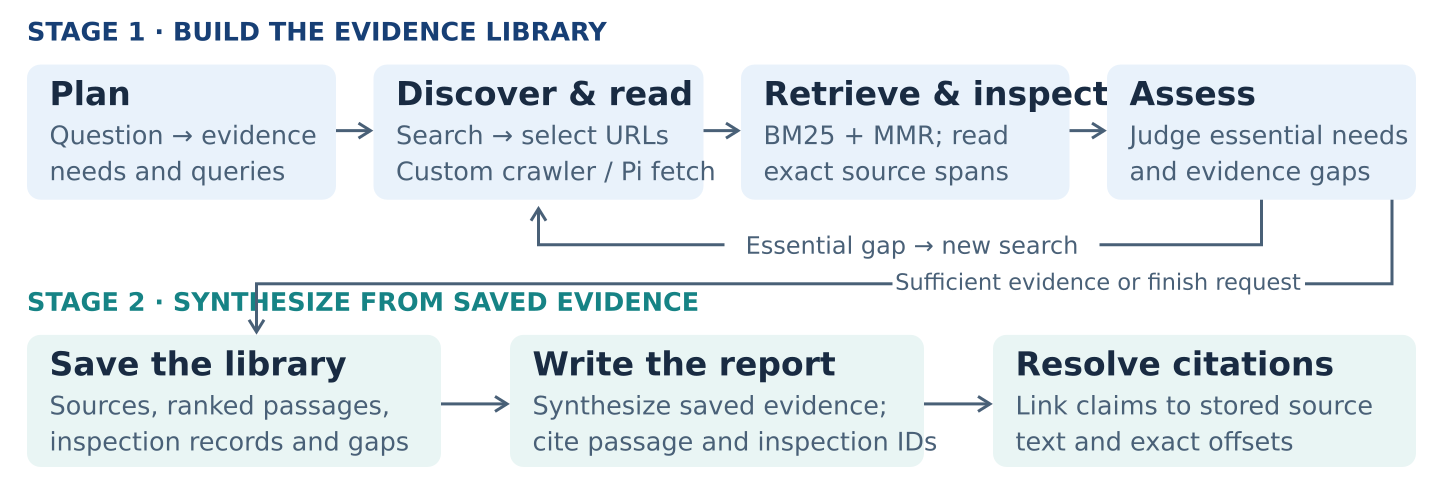
\includegraphics[width=.86\textwidth]{workflow.png}
\caption{Evidence-first research: discovery and source inspection can repeat; synthesis starts from the saved evidence, not the search transcript.}
\label{fig:workflow}
\end{figure*}
The pipeline in Fig.~\ref{fig:workflow} has two stages. The first plans evidence needs and builds a library: search, select, read, segment, rank, inspect, and assess. Essential gaps may trigger targeted follow-up searches. The second saves the library and synthesizes the final report, resolving evidence IDs to source spans. In the native Pi workflow, \texttt{/research-finish} hands off to synthesis after the current turn rather than cancelling.

\textbf{Acquisition and resource control.} Structured search results provide URLs, titles and snippets. Candidate selection uses URL normalization and lexical relevance; a multinomial Naive Bayes candidate classifier and passage clustering support more inspectable filtering and evidence facets in the research engine. The custom crawler implements per-host pacing, validated public-IP connections and redirects, HTML/PDF extraction, canonical metadata and explicit failure reasons. The budgeted engine additionally implements SQLite-backed resource accounting, protected synthesis capacity and retained-corpus follow-up. The live one-command report experiments use Pi's \texttt{fetch\_content} reader instead of racing both readers. Both approaches preserve extracted text and provenance; the live results do not validate every resource-control or multi-turn feature.

\section{Methodology}
\subsection{Passage Construction and Source Integrity}
The retrieval index packs paragraphs toward 180--300 surface tokens, with a 4,000-character cap and bounded overlap. It preserves UTF-16 source offsets in the retained extraction when it tokenizes or stems. URL normalization and shingle-based comparison reduce repeated evidence. The positional index uses five-token shingle Jaccard overlap; the live evidence library also uses shingle containment to help detect short renderings inside longer copies. Deduplication is heuristic and cannot make two reports of the same event independent. Only extracted page text enters the corpus, not search snippets or model-written summaries.

\subsection{Ranking and Feedback}
For query term $t$, passage $p$, passage count $N$, and document frequency $\mathrm{df}(t)$, the lexical score uses
\begin{equation}
\mathrm{IDF}(t)=\log\left(1+\frac{N-\mathrm{df}(t)+0.5}{\mathrm{df}(t)+0.5}\right),
\end{equation}
\begin{equation}
\sum_{t\in q}w(t,q)\,\mathrm{IDF}(t)\frac{(k_1+1)\,\mathrm{tf}(t,p)}{\mathrm{tf}(t,p)+k_1(1-b+b|p|/\overline{|p|})},
\end{equation}
with $k_1=1.2$, $b=0.75$. The positional ranker can add phrase/proximity signals. The parallel Porter-stemmed stream changes lexical matching, not source offsets. The BrowseComp-Plus runs rank a parent document $D$ by $\max_{p\in D}\mathrm{BM25}(q,p)$ and return unique documents. The live workflow uses MMR, greedily maximizing $\lambda \widetilde{s}(p)-(1-\lambda)\max_{p'\in S}\cos(v_p,v_{p'})$; the live library sets $\lambda=0.7$. This is not the same as the max-passage ablation. Dirichlet query likelihood, the sequential dependence model and lexical pseudo-relevance feedback are additional offline rankers; explicit positive/negative relevance feedback is available in the research engine.

\subsection{Synthesis and Scoped Checks}
A ranked shortlist can retrieve positive evidence but cannot establish absence. Direct inspection can count literal terms or return a specified source span; records include the source version, offsets and observed result. A scan of an incomplete extraction or a summary does not certify absence from an original paper. For open-ended claims, failures to fetch are recorded separately from what a search actually did not find. Citation IDs link to recorded evidence; semantic entailment is not guaranteed by link resolution.

\section{Experimentation and Results}
\subsection{End-to-End Deep Research and Judge Validation}
We built a project-specific harness on the official DeepResearch Bench prompts and point-wise RACE rubric~\cite{drb}. The judge, DeepSeek V4.1 Flash at temperature zero, receives one task, one candidate report and task-specific criteria in an independent call. It does not see human scores or a reference answer; criterion weights are applied after scoring. Weighted criterion means define comprehensiveness, insight, instruction following and readability scores; official dimension weights combine them on a 0--100 scale. The harness preserves raw responses and parsed scores. It does not verify claims against sources.

To validate the judge, we averaged three expert ratings and selected the human-best and human-worst system reports on each of 50 Chinese tasks (100 reports). It ordered the two reports correctly on \textbf{44/50 tasks (88\%)}; pooled Pearson $r=0.462$, within-task centered $r=0.690$, and raw MAE was 13.71 points. Per-dimension calibration cross-validated by task produced 10.72 MAE. Selection uses pairs with strong human separation, so this does not establish performance on close pairs. It supports same-task ranking more strongly than interpreting scores as absolute human ratings. The calibration does not validate English tasks, and the live generator and judge share a model family.

\begin{table}[t]
\caption{Same-task report quality under the project RACE judge (/100).}
\label{tab:race}
\centering\footnotesize
\begin{tabular}{lrr}
\toprule
\rowcolor{lightblue} System & Task 19 & Task 20 \\
\midrule
\textbf{Pi Research} & \textbf{94.29} & \textbf{83.04} \\
OpenAI Deep Research & 77.69 & 79.08 \\
drsh & 76.87 & 51.96 \\
Perplexity Research & 49.07 & -- \\
Grok Deeper Search & -- & 58.53 \\
\bottomrule
\end{tabular}
\end{table}
\begin{figure*}[t]
\centering
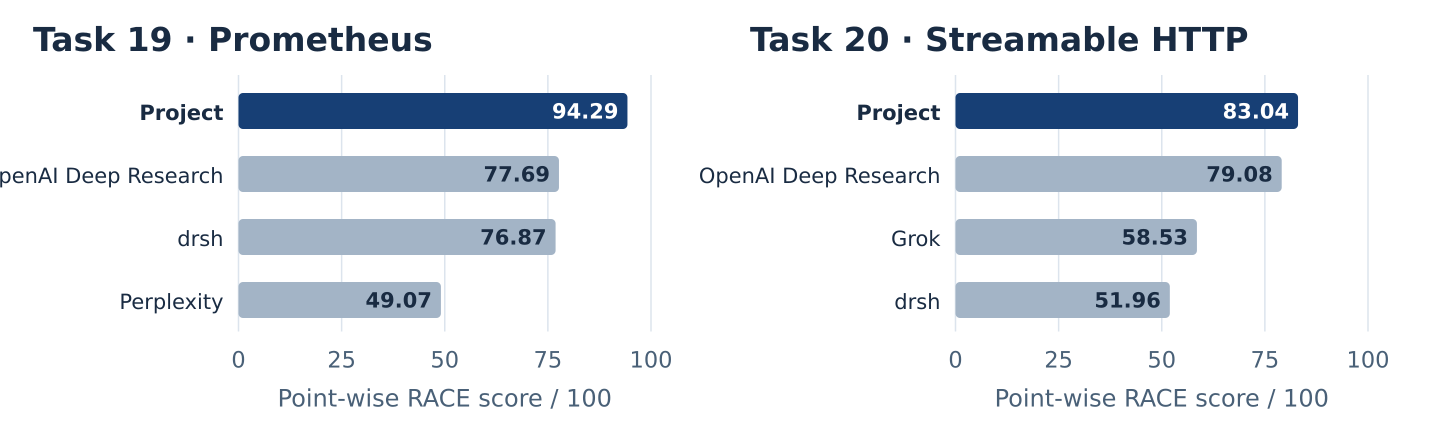
\includegraphics[width=.86\textwidth]{race-scores.png}
\caption{Report scores on Prometheus (Task 19) and Streamable HTTP (Task 20). Comparisons are within each task only; available baselines differ.}
\label{fig:race}
\end{figure*}
\textbf{Main result.} On the two scored tasks without detected published-answer leakage, Pi Research ranked first among the available same-task reports (Table~\ref{tab:race}, Fig.~\ref{fig:race}). It scored 16.60 and 3.96 points above the available OpenAI Deep Research report, respectively. These are two task results, not an aggregate leaderboard claim. Two further exploratory runs scored 75.32 (water utilities, Task 12) and 90.21 (low-code/no-code, Task 17), but both retrieved a publicly indexed answer to the exact benchmark task. We exclude both from fair comparisons.

\subsection{BrowseComp-Plus Evidence Retrieval}
The controlled retrieval experiment uses all 100,195 documents (2,282,733 passages), and 100 of 830 questions selected deterministically with seed 42 before retrieval. The subset has 595 evidence and 282 gold document judgments. Queries are used verbatim; no model or query rewrite participates. We score TREC runs against evidence and gold judgments separately. Gold documents contain the answer in addition to being relevant evidence. Recall is calculated against the judged pool, not all relevant web pages. nDCG@10 normalizes rank-discounted gain against an ideal ordering.

\begin{table*}[t]
\centering\footnotesize
\caption{BrowseComp-Plus retrieval (\%). The published full-set baseline is context, not a matched comparison.}
\label{tab:browsecomp}
\setlength{\tabcolsep}{5pt}
\begin{tabular}{lcrrrrrrrr}
\toprule
\rowcolor{lightblue} & & \multicolumn{4}{c}{Evidence judgments} & \multicolumn{4}{c}{Gold judgments} \\
\cmidrule(lr){3-6}\cmidrule(lr){7-10}
Method & Queries & R@5 & R@100 & R@1000 & nDCG@10 & R@5 & R@100 & R@1000 & nDCG@10 \\
\midrule
Published BM25~\cite{browsecomp} & 830 & 1.20 & 4.70 & 13.70 & 1.60 & 1.40 & 6.10 & 17.30 & 1.70 \\
Whole-document, Lucene-style & 100 & 1.56 & 4.17 & 15.16 & 2.13 & 0.50 & 4.83 & 22.33 & 1.03 \\
Whole-document BM25 & 100 & 2.51 & 9.50 & 28.25 & 3.70 & 3.50 & 15.48 & 35.93 & 3.86 \\
Passage BM25 & 100 & \textbf{5.87} & 21.32 & \textbf{46.24} & \textbf{8.47} & 7.36 & 26.75 & \textbf{50.55} & \textbf{8.75} \\
Porter-stemmed passage BM25 & 100 & 5.21 & \textbf{22.37} & 45.70 & 8.16 & \textbf{8.69} & \textbf{28.39} & 47.86 & 8.46 \\
\bottomrule
\end{tabular}
\end{table*}
\begin{figure*}[t]
\centering
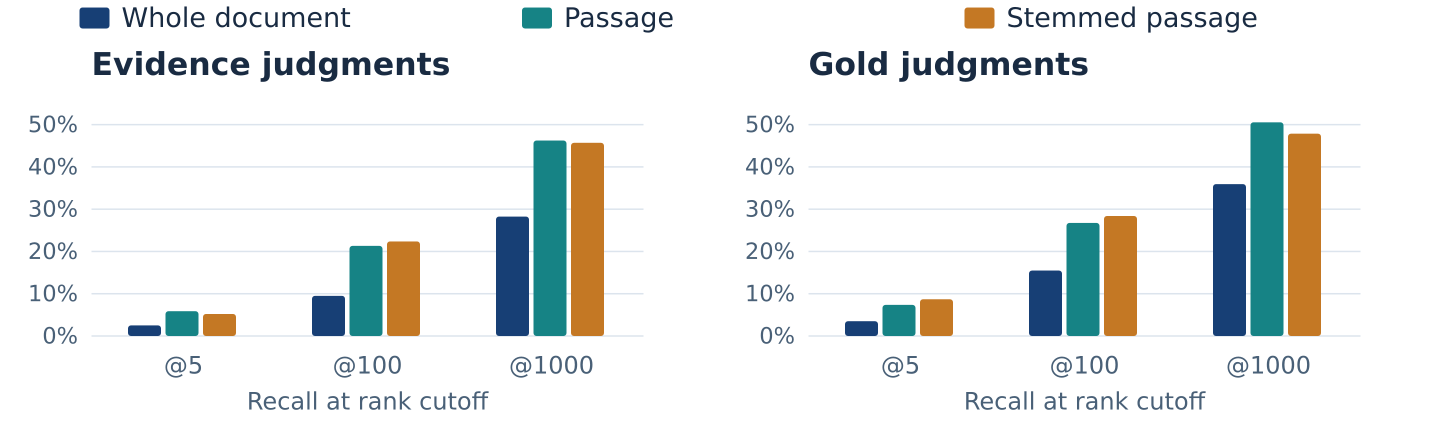
\includegraphics[width=.86\textwidth]{browsecomp-recall.png}
\caption{Recall across cutoffs for matched 100-query runs on the full BrowseComp-Plus corpus.}
\label{fig:recall}
\end{figure*}
Against whole-document BM25 with identical parameters, passage BM25 improves evidence Recall@1000 by 17.99 points (paired two-tailed $p=1.28\times10^{-11}$) and evidence nDCG@10 by 4.77 points ($p=0.0022$; Table~\ref{tab:browsecomp}, Fig.~\ref{fig:recall}). Stemming gives higher Gold Recall@5 (8.69\% versus 7.36\%), but its gains and losses against unstemmed passage scoring are not significant on this sample. Reported tests are unadjusted; evidence Recall@1000 and nDCG@10 still meet a conservative $0.05/8$ threshold. The published 830-query BM25 result uses a different analyzer and is not directly comparable to the 100-query project rows.

\subsection{CISI Retrieval Ablation}
The secondary retrieval experiment uses 1,459 indexed scientific abstracts and 76 judged queries. Precision at $k$ is the relevant fraction of the first $k$ results; pooled recall is the fraction of judged relevant documents retrieved. The project comparison in Table~\ref{tab:cisi} indicates that stemming improves early precision and nDCG on this corpus, whereas blind lexical feedback degrades ranking. This contrasts with the non-significant stemming differences on BrowseComp-Plus. The archived CISI per-query file covers the original BM25 and PRF variants; extended rows come from the team's reported evaluation. No CISI significance claim is made here because the extended per-query output was not validated in this report.

\begin{table}[t]
\centering\footnotesize
\caption{CISI mean retrieval scores on 76 judged queries.}
\label{tab:cisi}
\begin{tabular}{lrrrr}
\toprule
\rowcolor{lavender} Method & P@5 & P@10 & R@10 & nDCG@10 \\
\midrule
Stemmed BM25 & \textbf{.4263} & \textbf{.3632} & \textbf{.1470} & \textbf{.3984} \\
Plain BM25 & .3895 & .3105 & .1360 & .3607 \\
Dirichlet QL & .3684 & .2921 & .1392 & .3390 \\
SDM & .3605 & .2921 & .1275 & .3338 \\
Lexical PRF & .2974 & .2566 & .0955 & .2902 \\
Lexical PRF + MMR & .2868 & .2474 & .0915 & .2821 \\
\bottomrule
\end{tabular}
\end{table}

\subsection{Live Provenance Case Study}
For ``What is PMCR in medical image segmentation?'', an earlier run produced 6,173 words from secondary renderings, whose numerical claims conflicted. A later run acquired \href{https://arxiv.org/html/2406.05054v1}{109,282 characters of the original arXiv paper} through Pi's reader and produced a 785-word report with all 36 inline citation links resolving. The later run used \texttt{/research-finish} and took 6 minutes 50 seconds. It is an observed example of a provenance improvement, not a controlled speed comparison or evidence of general citation accuracy.

\section{Conclusions and Limitations}
Pi Research combines inspectable passage retrieval, controlled acquisition, a saved evidence library and a separate cited writing stage. The retrieval ablation supports passage scoring, and the two clean same-task report comparisons are the strongest end-to-end result. Neither establishes that the retrieval gain caused the higher report scores. Browser access and extraction can fail; deduplication and literal scans are incomplete; and a resolving citation need not support a claim. Published answers can contaminate open-web benchmarks. A larger leakage-screened evaluation, independent claim checking, and controlled multi-turn trials are needed before generalizing.

\section*{Reproducibility and Credits}
The submission includes the source, project PDF, DeepResearch Bench questions and criteria, judge outputs, and dataset links. The offline retrieval runs use the \href{https://ir.dcs.gla.ac.uk/resources/test_collections/cisi/}{Glasgow CISI collection} and \href{https://huggingface.co/datasets/Tevatron/browsecomp-plus-corpus}{BrowseComp-Plus}; the latter's large corpus is available from its official dataset repository. The \href{https://huggingface.co/datasets/muset-ai/DeepResearch-Bench-Dataset}{DeepResearch Bench dataset} supplies task prompts, rubrics and baseline articles. AI assistance supported code, analysis and report drafting; measured results, diagnostics, and unsupported comparisons are distinguished above.

\begin{thebibliography}{00}
\bibitem{bm25} Robertson, S. and Zaragoza, H., 2009. The probabilistic relevance framework: BM25 and beyond. \emph{Foundations and Trends in Information Retrieval}, 3(4), pp. 333--389.
\bibitem{porter} Porter, M.F., 1980. An algorithm for suffix stripping. \emph{Program}, 14(3), pp. 130--137.
\bibitem{mmr} Carbonell, J. and Goldstein, J., 1998, August. The use of MMR, diversity-based reranking for reordering documents and producing summaries. In \emph{Proceedings of the 21st Annual International ACM SIGIR Conference} (pp. 335--336).
\bibitem{ql} Zhai, C. and Lafferty, J., 2001. A study of smoothing methods for language models applied to ad hoc information retrieval. In \emph{Proceedings of the 24th Annual International ACM SIGIR Conference} (pp. 334--342).
\bibitem{sdm} Metzler, D. and Croft, W.B., 2005. A Markov random field model for term dependencies. In \emph{Proceedings of the 28th Annual International ACM SIGIR Conference} (pp. 472--479).
\bibitem{rag} Lewis, P., Perez, E., Piktus, A. et al., 2020. Retrieval-augmented generation for knowledge-intensive NLP tasks. In \emph{Advances in Neural Information Processing Systems}, 33.
\bibitem{mtrag} Katsis, Y., Rosenthal, S., Fadnis, K. et al., 2025. MTRAG: A multi-turn conversational benchmark for evaluating retrieval-augmented generation systems. \emph{Transactions of the Association for Computational Linguistics}, 13, pp. 784--808.
\bibitem{browsecomp} Chen, Z., Ma, X., Zhuang, S. et al., 2026, July. BrowseComp-Plus: A fair and disentangled evaluation benchmark for deep search agents. In \emph{Proceedings of the 64th Annual Meeting of the Association for Computational Linguistics (Volume 1)} (pp. 22349--22370).
\bibitem{drb} Du, M., Xu, B., Zhu, C., Zhang, L., Wang, X. and Mao, Z., 2026. DeepResearch Bench: A comprehensive benchmark for deep research agents. In \emph{Proceedings of the 14th International Conference on Learning Representations}.
\end{thebibliography}
\end{document}
